\chapter{Generalized Coordinates}
\label{chap:generalized-coordinates}

A particle system's \emph{configuration} encapsulates all positional information of said system, \ie{} the position of every particle in the system. Similarly, the \emph{configuration space} of a system models all of its possible configurations. For a system of ${n}$ particles in two dimensions, we can write the particles' position vectors as
%
\begin{equation*}
  \vec{r}_i = \begin{pmatrix} x_i \\ y_i \end{pmatrix} \in \mathbb{R}^2, \qquad i = 1, \ldots, n.
\end{equation*}
%
If all particles can move freely in both dimensions, \ie{} all ${\vec{r}_i}$ can be chosen arbitrarily, the system has ${m = 2n}$ \emph{degrees of freedom}. In many scenarios, however, the system is subject to \emph{constraints}, restricting the movement of particles by introducing dependencies between the particles' positions. If one were to pick arbitrary positions ${\vec{r}_i}$, one might end up violating some of these constraints. For now, let us assume constraints to depend only on the particles' positions and to be of the form
%
\begin{equation}
  f(\vec{r}_1, \ldots, \vec{r}_n) \stackrel{!}{\equiv} 0.
  \label{eqn:holonomic-constraint}
\end{equation}
%
In theoretical physics, constraints of this form are known as \emph{holonomic constraints}. The number of degrees of freedom in a constrained particle system is reduced by independent holonomic constraints \cite{Henneaux}. Other forms of constraints may not necessarily decrease the number of degrees of freedom in the system.

\emph{Generalized coordinates} are independent variables uniquely determining a constrained system's configuration that implicitly satisfy all of the system's holonomic constraints. Given a constrained particle system, one can find as many independent variables determining its configuration as there are degrees of freedom in said system. The number of generalized coordinates required to be able to describe all configurations satisfying the constraints is equal to the number of degrees of freedom in the system; however, their concrete choice is generally not uniquely determined \cite{Muehlleitner, Fliessbach}.

Considering the generalized coordinates uniquely determine the system's configuration, each particle's position can be written as a function of the generalized coordinates:
%
\begin{equation*}
  \vec{r}_i = \vec{r}_i(q_1, \ldots , q_m) \in \mathbb{R}^2
\end{equation*}
%
Note that for unconstrained particle systems, one could choose Cartesian coordinates ${(x_i, y_i) \in \mathbb{R}^2}$ as generalized coordinates, but is in no way forced to do so.





\subsection*{Example: Mechanical Pendulum}
A mechanical pendulum is a weight hanging from a pivot point by a rigid rod of length ${l}$, allowing it to swing. Due to the rod being rigid, the weight's movement is restricted to a circle of radius ${l}$ around the pivot point. When choosing the coordinate system such that the origin lies in the pivot point, we can express this restriction and dependency between the weight's ${x}$ and ${y}$ coordinates as
%
\begin{equation}
  f(x,y) = x^2 + y^2 - l^2 \;\stackrel{!}{\equiv}\; 0.
  \label{eqn:pendulum-constraint}
\end{equation}

\begin{figure}[H]
  \centering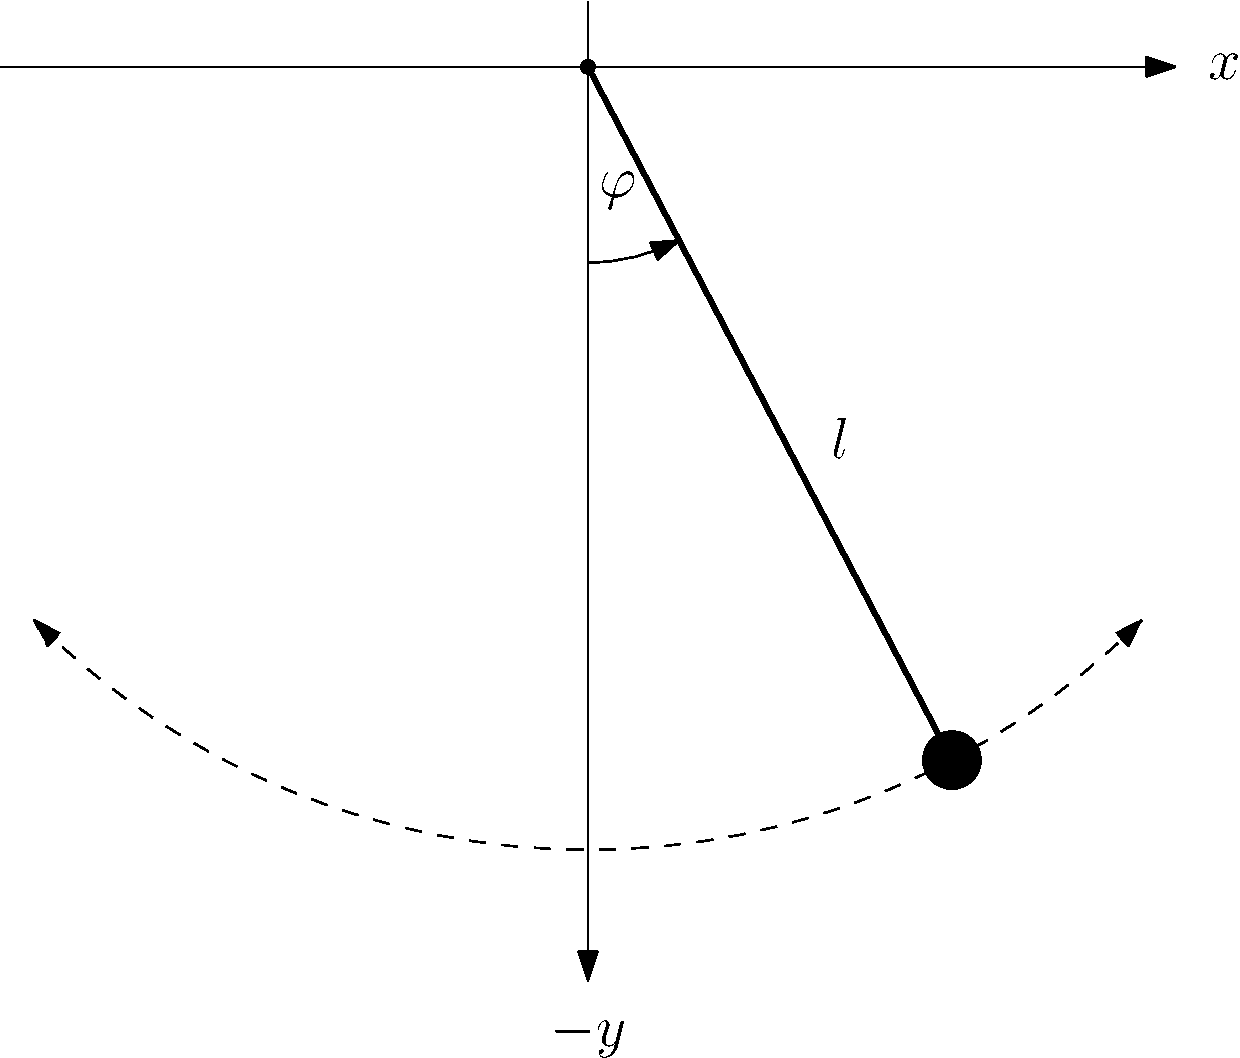
\includegraphics[width=0.5\textwidth]{Resources/Figures/Mechanical-Pendulum.pdf}
  \caption{A mechanical pendulum.}
  \label{fig:generalized-coordinates-for-pendulum}
\end{figure}

\noindent
Introducing a single generalized coordinate ${\varphi}$ determining the angular position of the weight relative to the vertical axis allows us to get rid of both ${x}$ and ${y}$, as they can now be written as a function of ${\varphi}$:
%
\begin{equation*}
  \vec{r}
  = \begin{pmatrix} x \\ y \end{pmatrix}
  = \begin{pmatrix*}[r] l \cdot \eval{\sin}{\varphi} \\ -l \cdot \eval{\cos}{\varphi} \end{pmatrix*}
\end{equation*}
%
With only one generalized coordinate ${\varphi}$, we can now express exactly those configurations that satisfy \cref{eqn:pendulum-constraint}.
